In the previous section we established the terminology we will use
throughout the document. This terminology will also be used to
decompose our system that solves the problem at hand, viz. that
we will model our solution according to the problem domain.

Specifically, we will create a system such that when we take in a
32-bit integer representing a valid or semi-valid MIPS32-instruction
then we can construct an object instance named \mij{Instruction} that
knows, or can retrieve information about,\footnote{Using its
collaborators}

\begin{table}
\begin{itemize}
\item Its numerical representation
\item Its own format
\item Its own decomposed representation presented in both:
\subitem Hexadecimal form
\subitem Decimal form
\item Its own mnemonic representation
\end{itemize}
\caption{\mij{Instruction} operations/fields}
\label{table:instruction-operations}
\end{table}
The \mij{Instruction} class is an abstraction providing an
encapsulation around the aforementioned points. Ultimately, the system
will be divided into the self-explanatory constituents

\begin{itemize}
\item \formatm: R, I, J
\item \opcodem: An abstraction around the numerical opcode.
\item \formatm: Can for a given \opcodem return the associated format.
\item \decomposedm: Can decompose a 32-bit number into varying lengths.
\item \registerm: Associates a number with the register name, see Table.~\ref{table:mips-register-naming-convention}
\end{itemize}

The manner with which we determine the particular instruction, and
yield the correct output, becomes very closely related to our original
example for the \tt{mul} instruction. In the following example we will
parse another R-type instruction, namely \tt{sub}, this time
explaining the process by following the code path.

\subsection{Example: Decomposing \texttt{sub}}

Consider the 32-bit integer \tt{0x00012122}. In this example, we will
parse the number in a sequence of steps, before finally arriving at
that this number represents an instance of the \tt{sub} instruction.

In an earlier section we established the input and output of our
decompiler, see Fig.~\eqref{fig:mips32-decompiler} which maps nicely
into Table.~\ref{table:instruction-operations}. In this example we
will start by supplying our factory
method \mij{Instruction.fromInteger(int instruction}} with
\tt{0x00012122} and evaluate the 

\begin{figure}[H]
  \centering 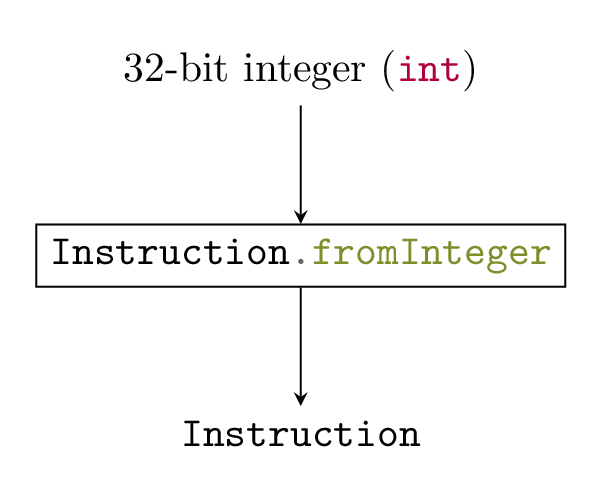
\includegraphics[width=0.7\textwidth]{figures/mips32-decompiler-interface.png} \caption{Interface} \label{fig:mips32-decompiler-interface}
\end{figure}


\subsubsection{Determining \texttt{Opcode} from a 32-bit integer}
First, we have that the \tt{Opcode} may be determined by the 6
left-most bits of the number, hence we would like to have a function
$f$ such that,

\begin{equation*}
f: \textrm{32-bit integer} \to \tt{Opcode}
\end{equation*}

In Java we can represent this by having a class, \opcodem\footnote{
\tt{src/main/java/se.filipallberg.dark.mips32decompiler.instruction.util.Opcode}}
with the method,

\begin{minted}{java}
public static Opcode fromInstruction(int instruction);
\end{minted}

The \opcodem abstraction will intermittently be represented in
numerical form, so in this
case \mintinline{java}{Opcode.fromInstruction(0x00012122)} will
occassionally be written out as \tt{0x00}. The class, \opcodem,
supplies handy utility methods for representing itself either as an
object or the \mij{int} primitive.

\subsubsection{Determining the \texttt{Format} from an \texttt{Opcode}}

As previously stated, for any defined \opcodem the format of the
instruction with that opcode is always known. I.e. there is a
one-to-one function (i.e. a mapping) that pairs an \mij{Opcode} with
a \mij{Format}.



\subsubsection{Identifying the instruction using the \texttt{Format}}

Before we stated that the \opcode is not always adequate to uniquely
identify the instruction. We find that all J-type instructions and for
some, but not all, I-type instructions the \opcode will suffice.
Specifically, those I-type instructions which cannot be identified by
their opcode alone is the branch instructions and immediate trap
operations.\footnote{For the opcodes \tt{op=0x00}, \tt{op=0x01},
and \tt{op=0x1c} it is necessary to consult a second field in order to
identify the instruction completely (\tt{funct} in the case
of \tt{op=x00} or \tt{ox1c} and
\tt{rt} in the case of \tt{op=0x01})}

\subsubsection{Review}

So far we have retrieved the \opcodem from \tt{0x00012122}, and from
the
\opcodem we got the \formatm.

%In turn, the \formatm gave us both the \decomposedm and the \inamem.

\subsection{Example: Decomposing \tt{sub} (continued)}

Before the above review we retrieved the \decomposedm. A \decomposedm
can represent itself in different bases, specifically in hex and decimal,
as a \mij{String}.

\begin{minted}{haskell}
hex :: DecomposedRepresentation -> String
decimal :: DecomposedRepresentation -> String
\end{minted}

where if we apply \mi{haskell}{hex} to the \decomposedm we have
we get \tt{[0 0 1 4 4 0x22]}.\footnote{Remember that an R-type instruction
decomposes into bitfields of length $(6, 5, 5, 5, 5, 6)$} and applying
\mintinline{haskell}{decimal} yields \tt{[0 0 1 4 4 34]}.

Recall from Fig. \ref{fig:mips32-decompiler} that for any 32-bit integer
representing a valid MIPS32-instruction the output we intend to produce is

\begin{itemize}
  \item The supplied 32-bit integer
  \item the format of the instruction
  \item the hexadecimal and decimal decomposed representation
  \item the mnemonic representation using register
          abbreviations wherever possible, and using decimal numbers
          when actual numbers are necessary.
\end{itemize}

We have docked off the first three items, and only getting the
mnemonic representation remains.\footnote{The first item is trivial}

\subsubsection{Mnemonic patterns}

We have not covered this before but the mnemonic representation of
instructions in the MIPS32 instruction set has a tendency to follow
a certain pattern, and these patterns are dependent upon the format of
the particular instruction.

For an example, the instructions

\begin{verbatim}
add, addu, sub, mul, and, or, nor, xor, movn, movz
\end{verbatim}

among possibly others, have the common pattern \emph{$\langle$iname
rd, rs, rt$\rangle$} with
\emph{iname} the instruction name.

\newcommand{\pattern}[1]{\emph{$\langle$#1$\rangle$}}

Other common patterns include 

\begin{itemize}
\item \pattern{iname rd, rs}
\item \pattern{iname rd, rt, rs}
\item \pattern{iname, rd, rt, shamt}
\end{itemize}

for R-format instructions and

\begin{itemize}
\item \pattern{iname, rt, rs, imm}
\item \pattern{iname rt, imm}
\item \pattern{iname, rt, rs(addr)}
\end{itemize}

for I-format instructions.

%Each \inamem is associated with a particular \pattern! We will call
these patterns a \mij{MnemonicPattern}, so we have that

\begin{minted}{haskell}
getMnemonicPattern :: InstructionName -> MnemonicPattern
\end{minted}

and that a \mij{MnemonicPattern} when applied to a \decomposedm
yields a \mij{Mnemonic}.\footnote{This is just a type synonym for a \texttt{String}}

\begin{minted}{haskell}
getMnemonicRepresentation :: InstructionName -> MnemonicPattern -> 
            DecomposedRepresentation -> MnemonicRepresentation
\end{minted}

\subsection{An decompilation algorithm}

Using the functions expressed in the previous sections we are now ready to
define an algorithm for our 32-bit integers.

\LetLtxMacro\i\textit
\newcommand{\get}[2]{\tt{#1} \i{#2} $\gets$ }
\newcommand{\of}[1]{(\i{#1})}
\newcommand{\from}[1]{\i{#1}}

\begin{algorithm}
\caption{Parsing/Decompilation algorithm}\label{algo:decompile}
\begin{algorithmic}[1]
\Procedure{Parse}{32-bit integer \i{int}}
\State \get{Opcode}{o}\from{getOpcode}\of{int}
\State \get{Format}{format}\from{getFormat}\of{o}
\State \get{InstructionName}{iname}\from{getName}\of{format, int}
\State \tt{DecomposedRepresentation} d
\State \get{}{d}\from{getDecomposedRepresentation}\of{format, int}
\State \get{String}{dec}\from{decimal}\of{d}
\State \get{String}{hex}\from{hex}\of{d}
\State \get{MnemonicPattern}{r}\from{getMnemonicPattern}\of{iname}
\State \tt{MnemonicRepresentation} mnemonic
\State \get{}{mnemonic}\from{getMnemonicRepresentation}\of{iname, r, d} \\
\Return (int, format, dec, hex, mnemonic)
\EndProcedure
\end{algorithmic}
\end{algorithm}



